\chapter{validação do SUpervisório Didático}

Nesta seção, serão utilizados 2 controladores devidamente sintonizados em um sistema simulado, cujas equações descritivas são conhecidas. No supervisório didático, existem mecanismos que simulam um controlador, sendo a finalidade deste processo validar os valores retornados pelo arduino, como respostas dos sinais de controle, e concluir sobre a empregabilidade do software supervisório.

\section{Apresentação do Sistema}

O sistema simulado pelo arduino se trata de dois tanques de área variável acoplados e alimentados por uma vazão controlável. A Figura \ref{img_sistema_teste} os esquematiza.

\begin{figure}[htb]
	\centering
	\caption{Esquema de leitura serial no supervisório didático}
	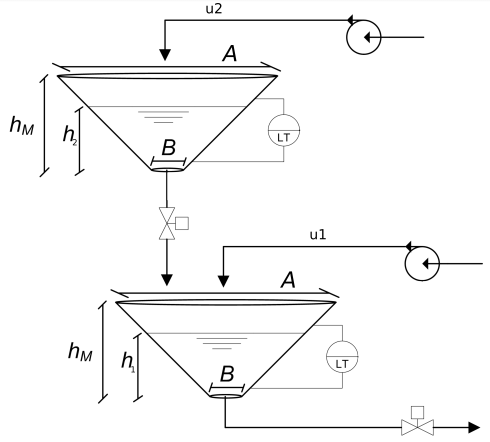
\includegraphics[width=0.8\textwidth,height=0.4\textheight]{sistema_teste}
	Fonte: Elaborado por \citeonline{santana2019}
	\label{img_sistema_teste}
\end{figure}

Os tanques têm o formato de tronco de cone e as variáveis controladas são suas alturas em metro. As variáveis manipuladas são as vazões de entrada de fluido em ambos os tanques.

As equações deste processo são descritas por
\begin{align}
\frac{dh_1}{dt} &= \frac{1}{\beta(h_1)}(u_1 - k\sqrt{\rho g h_1} + k\sqrt{\rho g h_2}) \\
\frac{dh_2}{dt} &= \frac{1}{\beta(h_2)}(u_2 - k\sqrt{\rho g h_2}) \\
\beta(h_i) &= \frac{dV}{dh_i} \\
V(h_i) &= \frac{\pi\gamma^2}{3}(h_i + \frac{B}{2\gamma})^3 - \frac{\pi}{3\gamma}(\frac{B}{2})^3 \\
\gamma &= \frac{A-B}{2h_M}
\label{eq_descritivas}
\end{align}
e seus parâmetros e variáveis são descritos e dimensionados na tabela \ref{tbl_parameters}:

\begin{table}[htb]
	\centering
	\caption{Tabela de parâmetros e variáveis do sistema}
	\begin{tabular} {|m{5em} m{15em} m{8em}|}
		\hline
		Símbolo & Descrição & Valor (u.m.) \\
		\hline
		$A$ & diâmetro superior & 4 (m) \\
		$B$ & diâmetro inferior & 1 (m) \\
		$hm$ & altura máxima & 4 (m) \\
		$V$ & volume & - (m\textsuperscript{3}) \\
		$h$ & altura & - (m) \\
		$\rho$ & densidade do fluido & 1000 (kg/m\textsuperscript{3}) \\
		$g$ & aceleração da gravidade & 9,8 (m/s\textsuperscript{2}) \\
		$k$ & constante de descarga no tanque & 0,001 (-)\\
		$u$ & vazão da bomba & - (m\textsuperscript{3}/s)\\
		\hline
	\end{tabular}
	\label{tbl_parameters}
\end{table}

\section{Comportamento esperado} \label{comportamento_esperado}

Por se tratar de um sistema não linear, pouco pode-se dizer de seu comportamento dinâmico, partindo-se somente das equações. Porém, pode-se prever possíveis estados estacionários, atingidos quando a taxa de variação dos estados no tempo é nula.

Com as derivadas zeradas nas equações descritivas \ref{eq_descritivas}, tem-se que:
\begin{equation}
{h_1}_{ss} = (\frac{{u_1}_{ss}}{k\sqrt{\rho g}} + \sqrt{{h_2}_{ss}})^2
\end{equation}
\begin{equation}
{h_2}_{ss} = \frac{{u_2}_{ss}^2}{k^2 \rho g}
\end{equation}
, o que resultam em infinitos valores representando estados estacionários deste sistema. Para o processo de linearização, contemplado na próxima subseção, ao menos um ponto deve ser definidos. Partindo de um valor 0 para a vazão de alimentação do tanque 2, no topo, e uma altura final de 1 metro para o mesmo, calculam-se o restante dos estados estacionários na tabela \ref{tbl_ss}.

\begin{table}[htb]
	\centering
	\caption{Tabela de valores de um dos estados estacionário do sistema}
	\begin{tabular} {|m{5em} m{8em}|}
		\hline
		Variável & Valor (u.m.) \\
		\hline
		${h_1}_{ss}$ & 1 (m) \\
		${h_2}_{ss}$ & 1 (m) \\
		${u_1}_{ss}$ & 0 (m\textsuperscript{3}/s) \\
		${u_2}_{ss}$ & 0,099 (m\textsuperscript{3}/s)\\
		\hline
	\end{tabular}
	\label{tbl_ss}
\end{table}

Para validar estes valores, é possível usar o supervisório didático como auxílio. Para isto, programa-se o arduino para simular o sistema, partindo dos pontos na tabela \ref{tbl_ss}, enquanto que o módulo do controlador no programa envia os valores constantes de ${u_1}_{ss}$ e ${u_2}_{ss}$. Executada a simulação, a Figura \ref{img_ss} mostra o resultado. Nota-se a altura $h_2$ do sistema cai ao iniciá-lo, mas isso se deu ao atraso de comunicação entre o arduino e o computador. Mesmo assim, o sistema retorna para uma região próxima à que foi iniciado, momento no qual não apresenta outras variações significativas.

\begin{figure}[htb]
	\centering
	\caption{Sistema partido no estado estacionário}
	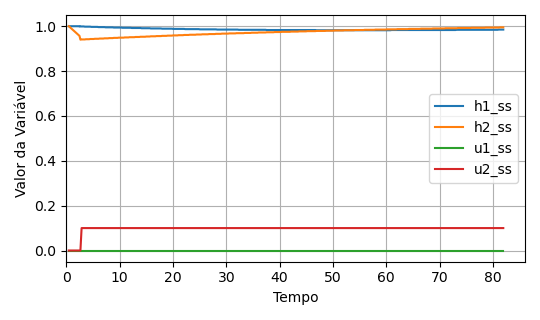
\includegraphics{estado_estacionario}
	\label{img_ss}
\end{figure}

\subsection{Linearização do Sistema}

Aplicando a linearização no sistema de estudo, as novas equações do sistema, em desvio, serão:
\begin{align}
\frac{dh_1}{dt} &= -\big(\frac{d\beta^{-1}(h)}{dh}\bigg|_{{h_1}_{ss}} k\sqrt{\rho g {h_1}_{ss}} + \frac{\beta^-1({h_1}_{ss}) k\sqrt{\rho g}}{2\sqrt{{h_1}_{ss}}}\big)\overline{h_1} + \big(\frac{\beta^-1({h_1}_{ss}) k\sqrt{\rho g}}{2\sqrt{{h_2}_{ss}}}\big)\overline{h_2} +  \beta^{-1}({h_1}_{ss})\overline{u_1} \\
\frac{dh_2}{dt} &= -\big(\frac{d\beta^{-1}(h)}{dh}\bigg|_{{h_2}_{ss}} k\sqrt{\rho g {h_2}_{ss}} + \frac{\beta^-1({h_2}_{ss}) k\sqrt{\rho g}}{2\sqrt{{h_2}_{ss}}}\big)\overline{h_2} + \beta^{-1}({h_1}_{ss})\overline{u_2} \\
\beta^{-1}(h) &= \frac{4}{4\pi(\gamma h)^2 + 4B\gamma h + B^2} \\
\frac{d\beta^{-1}(h)}{dh} &= -4 \frac{8 \pi \gamma^2 h + 4 \gamma B}{(4\pi(\gamma h)^2 + 4B\gamma h + B^2)^2} \\
\end{align}
Substituindo os estados estacionários da tabela \ref{tbl_ss} e os parâmetros da tabela \ref{tbl_parameters}, tem se:
\begin{align}
\overline{h_1(s)} = & \frac{0,046}{s + 0,063}\overline{h_2} + \frac{0,937}{s + 0,063}\overline{u_1} \\
\overline{h_1(s)} = & \frac{0,937}{s + 0,063}\overline{u_2}
\end{align}

Em formato de espaço de estados o sistema final linearizado será:
\begin{equation}
\begin{pmatrix} \dot{\overline{h_1}} \\ \dot{\overline{h_2}} \end{pmatrix} = \begin{pmatrix} -0,063 & 0,046 \\ 0 & -0,063 \end{pmatrix} \begin{pmatrix} \overline{h_1} \\ \overline{h_2} \end{pmatrix} + \begin{pmatrix} 0,937 & 0 \\ 0 & 0,937 \end{pmatrix} \begin{pmatrix} \overline{u_1} \\ \overline{u_2} \end{pmatrix}
\label{espaco_estados}
\end{equation}

\subsection{Sintonia do PI}

Para a sintonia do PI pelo método síntese, toma-se uma entrada para cada saída, pelo critério de maior impacto. Pela equação \ref{espaco_estados}, nota-se que a entrada $u_1$ tem maior impacto em $h_1$ e $u_2$ em $h_2$. Logo, os controladores, projetados para um tempo de resposta $\tau_c$ de 10 segundos, de acordo com a equação \ref{sintese_controlador}, serão:
\begin{equation}
C_1(s) = C_2(s) = \frac{1}{10s} \frac{s + 0,063}{0,937} = 0,1067 + 0,0067 \frac{1}{s}
\end{equation}

\subsection{Sintonia do LQR}

Para o presente caso de teste, partindo da equação \ref{espaco_estados}, tem-se como matrizes $A$ e $B$:
\begin{equation}
A = \begin{pmatrix} -0,063 & 0,046 \\ 0 & -0,063 \end{pmatrix},
B = \begin{pmatrix} 0,937 & 0 \\ 0 & 0,937 \end{pmatrix}
\end{equation}

Assumindo que nenhum estado nem entrada deve levar maior importância em relação aos outros, tem-se como matrizes de ganhos $Q$ e $R$
\begin{equation}
Q = \begin{pmatrix} 0,5 & 0 \\ 0 & 0,5 \end{pmatrix},
R = \begin{pmatrix} 0,5 & 0 \\ 0 & 0,5 \end{pmatrix}
\end{equation}
, que geram a matriz de ganho $K$:
\begin{equation}
K = \begin{pmatrix} 0,935 & 0,023 \\ 0,023 & 0,936 \end{pmatrix}
\end{equation}

De acordo com a equação \ref{lqr_generic_control_func}, as entradas do sistema serão então regidas pelas equações:
\begin{align}
\overline{u_1} &= 0,935 \overline{h_1} + 0,023 \overline{h_2} \\
\overline{u_2} &= 0,023 \overline{h_1} + 0,936 \overline{h_2}
\label{lqr_control_function}
\end{align}

A equação do LQR foi construída de acordo com o sistema linearizado. Assim, elas devem ser passadas para o controlador em formato de desvio.

\section{Configuração do supervisório didático}

Como já mencionado, o supervisório didático implementa duas funções que podem ser editadas pelo usuário, de forma que seja possível uma resposta ao dispositivo conectado, simulando um controlador. O usuário tem liberdade de escrever suas próprias funções e alterar os objetos do código-fonte como preferir, para atender às suas necessidades. As seguintes seções apresentam o código utilizado nas funções \emph{setup\_control()} e \emph{loop\_control()} para cada controlador escolhido.

\subsection{Controlador PI}

Além da biblioteca \emph{python-control}, existe outra chamada \emph{simple-pid} que, como o nome indica, possui objetos que se comportam como controladores PID. Eles recebem como parâmetros seus respectivos ganhos, valores de setpoints, limites para a resposta e outros que são referenciados \href{https://pypi.org/project/simple-pid/}{em sua documentação}, e tem sua funçao de controle descrita como a equação \ref{eq_PID}. Para implementá-los no programa, na função \emph{setup\_control()}, criam-se tais objetos de acordo com o código \ref{code_pi_setup}.

\begin{code}
\begin{lstlisting}
self.pids = []
self.pids.append(simple_pid.PID(0.1067, 0.0067, setpoint=2.5))
self.pids.append(simple_pid.PID(0.1067, 0.0067, setpoint=2.5))
\end{lstlisting}
\label{code_pi_setup}
\end{code}

O objeto PID da biblioteca simple-pid, quando chamado, retorna um valor numérico referente à resposta do controlador a partir de uma leitura, informada como parâmetro. Este valor pode ser escrito diretamente na porta serial, e será capturado pelo dispositivo conectado, desde que o mesmo esteja preparado para recebê-lo. No Arduino, o comando \emph{\textbf{Serial}.parseFloat()} lê a parte decimal do valor numérico presente na porta. Assim, foi preciso normalizar o sinal de controle, transformando um intervalo de valores que contenha qualquer valor possível seu (no caso, [0, 10] foi suficiente) em outro que possa ser lido pelo controlador ([0, 1]).

Implementa-se, então, na função \emph{loop\_control()}, o código \ref{code_pi_loop}:

\begin{code}
\begin{lstlisting}
	if len(input_data) == 0:
		return

	signals = [self.pids[i](input_value) for i, input_value in enumerate(input\_data)]
	for signal in signals:
		self.porta.write('{:.2f}'.format(signal/10).encode('UTF-8'))
	return
\end{lstlisting}
\label{code_pi_loop}
\end{code}

\subsection{LQR}

Uma das alternativas para a implementação do LQR no programa é a de usar a mesma biblioteca \emph{control} referenciada no Quadro \ref{qdr_used_libs}, que simula processos por funções de transferência. Nela existe a função \emph{lqr()} que retorna, entre outras saídas, a matriz de ganhos $K$ que parametriza a função de controle mostrada na equação \ref{lqr_generic_control_func}

Na função \emph{setup\_control()}, escreve-se o código \ref{code_lqr_loop}, onde calcula-se primeiramente a matriz de ganhos $K$ e a armazena como uma propriedade do objeto pai. Aqui também foram definidos os desvios das variáveis, que serão empregados no cálculo de cada sinal de controle.

\begin{code}
\begin{lstlisting}
A = [[-0.063, 0.046],[0, -0.063]]
B = [[0.937, 0],[0, 0.937]]
Q = [[0.5, 0],[0, 0.5]]
R = [[0.5, 0],[0, 0.5]]
K, P, V = control.lqr(A, B, Q, R)

rho = 1000
g = 9.8
k = 0.001

self.K = K
self.h1ss = 1
self.h2ss = 1
self.u1ss = 0
self.u2ss = k*math.sqrt(rho*g)

return
\end{lstlisting}
\label{code_lqr_loop}
\end{code}

Na função \emph{loop\_control()}, aplica-se a equação \ref{lqr_control_function} para o cálculo dos sinais de controle a cada iteração.

\begin{code}
\begin{lstlisting}
if len(input_data) == 0:
	print('No Read')
	return

#Transformacao em desvio
input_data[0] = input_data[0] - self.h1ss
input_data[1] = input_data[1] - self.h2ss

signals = [-(input_data[0]*self.K[0][0] + input_data[1]*self.K[0][1]) + self.u1ss,
		-(input_data[0]*self.K[1][0] + input_data[1]*self.K[1][1]) + self.u2ss]
for signal in signals:
	resp = '{:.3f}'.format(float(signal)/10).encode('UTF-8')
	self.porta.write(resp)
return
\end{lstlisting}
\label{code_lqr_loop}
\end{code}

\section{Validação dos dados}

Todos os casos de teste foram executados, e as séries foram salvas no programa, como mostrado na Figura \ref{img_series_salvas}.

\begin{figure}[htb]
	\centering
	\caption{Interface com as séries salvas}
	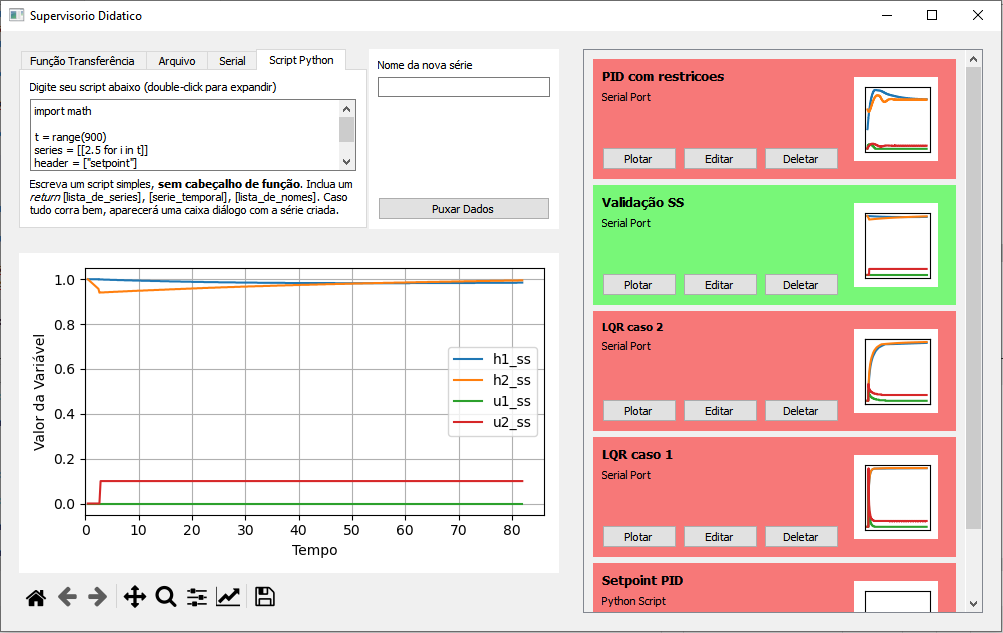
\includegraphics[width=\textwidth]{series_salvas}
	\label{img_series_salvas}
\end{figure}

Com isto, a os gráficos foram exportandos clicando em 
\includegraphics[height=1em]{save_icon} e copiados para este documento.

O código do Arduino encontra-se no Apêndice \ref{Chap:Apendice1}. Por simular o processo em si, foi incluído nele um trecho de código para limitar os estados e entradas nos seguintes critérios:

\begin{enumerate}
	\item As alturas ${h_1}_{ss}$ e ${h_2}_{ss}$ devem estar compreendidas no intervalo [0, 4]m
	\item As entradas do sistema assumem valores somente entre 0 e 1 $m^3/s$
\end{enumerate}

Com o script contendo os códigos \ref{code_pi_setup} e \ref{code_pi_loop}, a comunicação com o arduino foi testada e retornou sucesso. A caixa \emph{SCADADialog} apareceu sem grandes problemas. Foi constatado, em tempo real, como os estados do sistema adiquiriram um comportamento oscilatório, para depois suavemente atingirem os setpoints.

Se trantando do controlador PI, entretanto, o controle não foi perfeito, como constatado na Figura \ref{img_pid_com_restricoes}. Não somente o sistema levou cerca de 10 minutos para estabilizar, como também tem comportamento dinâmico oscilatório, o que não corresponde com o sistema de primeira ordem \emph{a priori} projetado.

\begin{figure}[htb]
	\centering
	\caption{Resposta do processo para controlador PI, incluindo restrições de processo}
	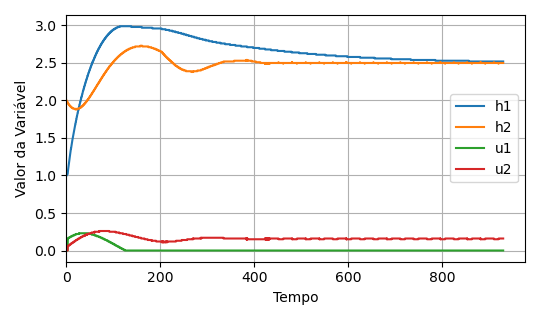
\includegraphics{PID_com_restricoes}
	\label{img_pid_com_restricoes}
\end{figure}

Nota-se que o sinal de controle foi corretamente saturado em 0, validando o limitador do sistema. O gráfico também é contínuo, sem falhas visíveis de comunicação ou leituras discrepantes. Através de um curto script Python foi criada uma linha reta "setpoint" no gráfico plotada em conjunto com os resultados.

Também para o caso do LQR não houveram interrupções ou leituras inesperadas durante o monitoramento. Percebeu-se que o sistema respondeu bem mais rápido que o do caso anterior, a custo de um maior esforço de controle.

\begin{figure}[htb]
	\centering
	\caption{Resposta do LQR no caso 1}
	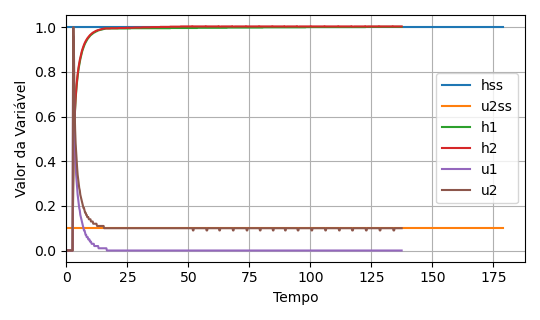
\includegraphics{LQR_caso_1}
	\label{img_lqr_caso_1}
\end{figure}

Como o de se esperar de um LQR, ocorre um pico no início da execução, que foi corretamente saturado. Após meio minuto de simulação, o sistema já se encontrava em estado estacionário.

Para dimunuir o esforço de controle, o peso de cada variável controlada foi aumentado de 0.5 para 5. Como constatado na Figura \ref{img_lqr_caso_2}, este objetivo foi, de fato, alcançado, e o sistema levou mais tempo para se acomodar, a troco de menor esforço das bombas.

\begin{figure}[htb]
	\centering
	\caption{Resposta do LQR no caso 2}
	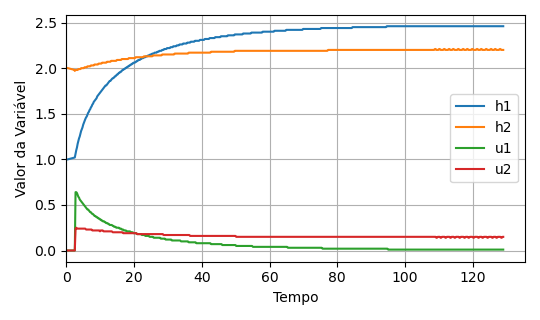
\includegraphics{LQR_caso_2}
	\label{img_lqr_caso_2}
\end{figure}

Ao salvar as séries de dados (Figura \ref{img_edit_lqr_caso_2}), observou-se no eixo de tempo que o período dos dados é de cerca de 0,2s, tempo satisfatório para simulação de sistemas químicos, que tendem a ser lentos. Porém, em aplicações reais, isto é um ponto a se avaliar, se se tornará um problema.

\begin{figure}[htb]
	\centering
	\caption{Resposta do LQR no caso 2}
	\includegraphics[width=\textwidth]{edit_LQR_caso_2}
	\label{img_edit_lqr_caso_2}
\end{figure}

\section{Considerações Finais}

Neste capítulo, foram simulados e comparados dois diferentes métodos de controle num sistema de tanques acoplados. No caso do PI, apesar de haver certa demora para regular o sistema, o esforço de controle não chegou perto do limite máximo, e o estado estacionário atingido foi bem próximo dos setpoints escolhido. Em contrapartida, o LQR apresentou um erro estacionário visível, e demandou um esforço maior de controle. Por outro lado, a sintonia de ambos são diferentes, e outros valores podiam ter sido empregados para $\tau$ do sistema final modelado para o PID.

No geral, pode-se afirmar que o supervisório didático cumpriu seu propósito em trazer os dados em tempo real e com confiança ao usuário. Não só isso, possibilitou que os gráficos de resposta fossem facilmente armazenados e exportados em formato de imagem. Um ponto de melhoria seria permitir que o setpoint fosse modificado em tempo de execução, para que o comportamento do sistema fosse perturbado. Por outro lado, isto pode ser feito com programação Python na função do loop de controle.